\textbf{Faça um esboço do Espectro de Magnitude do sinal amostrado por um trem de impulso.}

Considerando o espectro de um sinal de tempo contínuo $X(\omega)$ como:


\begin{figure}[H]
\centering

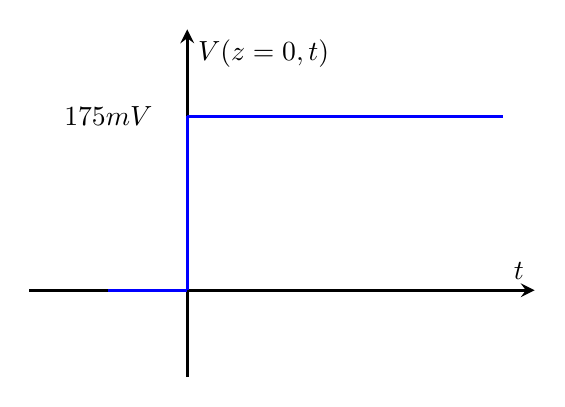
\begin{tikzpicture} 
\begin{axis}[very thick,
                     samples = 100,
                     ytick={-2,2},
                     xlabel = {$t$},
                     ylabel = {$V(z=0, t)$},
                     xmin = -1,
                     xmax = 2.2,
                     ymin = -0.5,
                     ymax = 1.5,
                     width=8cm,
                     height=6cm,
                     axis x line = middle,
                     axis y line = middle,
                     ticks = none]
                     
            \addplot[blue] coordinates {(-0.5,0) (0,0)};
            \addplot[blue] coordinates {(0,0) (0,1)};
            \addplot[blue] coordinates {(0,1) (2,1)};
            \node at (axis cs:-0.5,1){$175 mV$};
            
        \end{axis}
\end{tikzpicture}

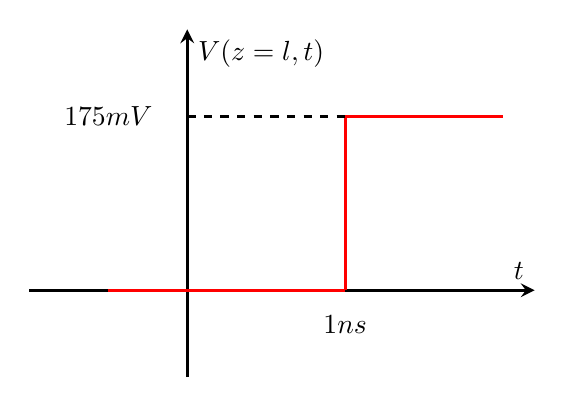
\begin{tikzpicture} 
\begin{axis}[very thick,
                     samples = 100,
                     ytick={-2,2},
                     xlabel = {$t$},
                     ylabel = {$V(z=l, t)$},
                     xmin = -1,
                     xmax = 2.2,
                     ymin = -0.5,
                     ymax = 1.5,
                     width=8cm,
                     height=6cm,
                     axis x line = middle,
                     axis y line = middle,
                     ticks = none]
                     
            \addplot[red] coordinates {(-0.5,0) (1,0)};
            \addplot[red] coordinates {(1,0) (1,1)};
            \addplot[red] coordinates {(1,1) (2,1)};
            \addplot[dashed] coordinates {(0,1) (1,1)};
            \node at (axis cs:-0.5,1){$175 mV$};
            \node at (axis cs:1,-0.2){$1ns$};
            
        \end{axis}
\end{tikzpicture}

\caption{First graph shows the voltage at the start of the line and the second shows the voltage at the end of the line. Source: own.}
\label{graph:1} 
\end{figure}

De acordo com a equação \ref{eq1:4}, o espectro de magnitude deste sinal amostrado por um trem de impulsos será:


\begin{figure}[H]
\centering
\tikz \node [scale=0.8, inner sep=0] {
\begin{tikzpicture} 
    \draw[black, very thick] (-2,3) -- (0,3);
    \draw[black, very thick] (0,3) -- (0,0);
    \draw[black, very thick] (0,0) -- (2,0);
    \node[blue] at (-2.4,3) {$R_{in}$};  
    \node[red] at (2.4,0) {$R_{L}$};  
    \node[black] at (1,1.5) {$1+Q_s^2$};  
    \draw[>=latex, <->] (0.2,0) -- (0.2,3);
    \node[black] at (0,-0.5) {(a)};
\end{tikzpicture}
};
\hspace{1cm}
\tikz \node [scale=0.8, inner sep=0] {
\begin{tikzpicture} [american]
    \draw[>=triangle 90, ->] (-0.5,0) -- (0.5,0);
    \draw[>=triangle 90, ->] (6.5,0) -- (5.5,0);
    \node[black] at (-0.9,0) {$R_{in}$}; 
    \node[black] at (6.9,0) {$R_L$}; 
    \node[black] at (3,-4) {(b)};
    \draw (1,0) to[L, l=$L$, *-*] (5,0)
    (2,0) to[C, l=$C$, *-] (2,-3) node[ground]{}
    ;
\end{tikzpicture}
};

\caption{(a) Desired effect of impedance gain(b) L matching network for a serial to parallel transformation of load impedance. Source: own.}
\label{graph:2} 
\end{figure}

Observa-se claramente pela figura \ref{graph:2} que a frequência de amostragem foi corretamente escolhida de acordo com o teorema de Nyquist-Shannon, ou seja, $\omega_s>2\pi B$. 
